% Options for packages loaded elsewhere
\PassOptionsToPackage{unicode}{hyperref}
\PassOptionsToPackage{hyphens}{url}
\PassOptionsToPackage{dvipsnames,svgnames,x11names}{xcolor}
%
\documentclass[
  12pt,
  a4paper,
]{scrreprt}

\usepackage{amsmath,amssymb}
\usepackage{iftex}
\ifPDFTeX
  \usepackage[T1]{fontenc}
  \usepackage[utf8]{inputenc}
  \usepackage{textcomp} % provide euro and other symbols
\else % if luatex or xetex
  \usepackage{unicode-math}
  \defaultfontfeatures{Scale=MatchLowercase}
  \defaultfontfeatures[\rmfamily]{Ligatures=TeX,Scale=1}
\fi
\usepackage{lmodern}
\ifPDFTeX\else  
    % xetex/luatex font selection
\fi
% Use upquote if available, for straight quotes in verbatim environments
\IfFileExists{upquote.sty}{\usepackage{upquote}}{}
\IfFileExists{microtype.sty}{% use microtype if available
  \usepackage[]{microtype}
  \UseMicrotypeSet[protrusion]{basicmath} % disable protrusion for tt fonts
}{}
\usepackage{xcolor}
\usepackage[left=3cm,,right=2cm,,top=3cm,,bottom=2cm]{geometry}
\setlength{\emergencystretch}{3em} % prevent overfull lines
\setcounter{secnumdepth}{5}

\usepackage{color}
\usepackage{fancyvrb}
\newcommand{\VerbBar}{|}
\newcommand{\VERB}{\Verb[commandchars=\\\{\}]}
\DefineVerbatimEnvironment{Highlighting}{Verbatim}{commandchars=\\\{\}}
% Add ',fontsize=\small' for more characters per line
\newenvironment{Shaded}{}{}
\newcommand{\AlertTok}[1]{\textcolor[rgb]{1.00,0.33,0.33}{\textbf{#1}}}
\newcommand{\AnnotationTok}[1]{\textcolor[rgb]{0.42,0.45,0.49}{#1}}
\newcommand{\AttributeTok}[1]{\textcolor[rgb]{0.84,0.23,0.29}{#1}}
\newcommand{\BaseNTok}[1]{\textcolor[rgb]{0.00,0.36,0.77}{#1}}
\newcommand{\BuiltInTok}[1]{\textcolor[rgb]{0.84,0.23,0.29}{#1}}
\newcommand{\CharTok}[1]{\textcolor[rgb]{0.01,0.18,0.38}{#1}}
\newcommand{\CommentTok}[1]{\textcolor[rgb]{0.42,0.45,0.49}{#1}}
\newcommand{\CommentVarTok}[1]{\textcolor[rgb]{0.42,0.45,0.49}{#1}}
\newcommand{\ConstantTok}[1]{\textcolor[rgb]{0.00,0.36,0.77}{#1}}
\newcommand{\ControlFlowTok}[1]{\textcolor[rgb]{0.84,0.23,0.29}{#1}}
\newcommand{\DataTypeTok}[1]{\textcolor[rgb]{0.84,0.23,0.29}{#1}}
\newcommand{\DecValTok}[1]{\textcolor[rgb]{0.00,0.36,0.77}{#1}}
\newcommand{\DocumentationTok}[1]{\textcolor[rgb]{0.42,0.45,0.49}{#1}}
\newcommand{\ErrorTok}[1]{\textcolor[rgb]{1.00,0.33,0.33}{\underline{#1}}}
\newcommand{\ExtensionTok}[1]{\textcolor[rgb]{0.84,0.23,0.29}{\textbf{#1}}}
\newcommand{\FloatTok}[1]{\textcolor[rgb]{0.00,0.36,0.77}{#1}}
\newcommand{\FunctionTok}[1]{\textcolor[rgb]{0.44,0.26,0.76}{#1}}
\newcommand{\ImportTok}[1]{\textcolor[rgb]{0.01,0.18,0.38}{#1}}
\newcommand{\InformationTok}[1]{\textcolor[rgb]{0.42,0.45,0.49}{#1}}
\newcommand{\KeywordTok}[1]{\textcolor[rgb]{0.84,0.23,0.29}{#1}}
\newcommand{\NormalTok}[1]{\textcolor[rgb]{0.14,0.16,0.18}{#1}}
\newcommand{\OperatorTok}[1]{\textcolor[rgb]{0.14,0.16,0.18}{#1}}
\newcommand{\OtherTok}[1]{\textcolor[rgb]{0.44,0.26,0.76}{#1}}
\newcommand{\PreprocessorTok}[1]{\textcolor[rgb]{0.84,0.23,0.29}{#1}}
\newcommand{\RegionMarkerTok}[1]{\textcolor[rgb]{0.42,0.45,0.49}{#1}}
\newcommand{\SpecialCharTok}[1]{\textcolor[rgb]{0.00,0.36,0.77}{#1}}
\newcommand{\SpecialStringTok}[1]{\textcolor[rgb]{0.01,0.18,0.38}{#1}}
\newcommand{\StringTok}[1]{\textcolor[rgb]{0.01,0.18,0.38}{#1}}
\newcommand{\VariableTok}[1]{\textcolor[rgb]{0.89,0.38,0.04}{#1}}
\newcommand{\VerbatimStringTok}[1]{\textcolor[rgb]{0.01,0.18,0.38}{#1}}
\newcommand{\WarningTok}[1]{\textcolor[rgb]{1.00,0.33,0.33}{#1}}

\providecommand{\tightlist}{%
  \setlength{\itemsep}{0pt}\setlength{\parskip}{0pt}}\usepackage{longtable,booktabs,array}
\usepackage{calc} % for calculating minipage widths
% Correct order of tables after \paragraph or \subparagraph
\usepackage{etoolbox}
\makeatletter
\patchcmd\longtable{\par}{\if@noskipsec\mbox{}\fi\par}{}{}
\makeatother
% Allow footnotes in longtable head/foot
\IfFileExists{footnotehyper.sty}{\usepackage{footnotehyper}}{\usepackage{footnote}}
\makesavenoteenv{longtable}
\usepackage{graphicx}
\makeatletter
\newsavebox\pandoc@box
\newcommand*\pandocbounded[1]{% scales image to fit in text height/width
  \sbox\pandoc@box{#1}%
  \Gscale@div\@tempa{\textheight}{\dimexpr\ht\pandoc@box+\dp\pandoc@box\relax}%
  \Gscale@div\@tempb{\linewidth}{\wd\pandoc@box}%
  \ifdim\@tempb\p@<\@tempa\p@\let\@tempa\@tempb\fi% select the smaller of both
  \ifdim\@tempa\p@<\p@\scalebox{\@tempa}{\usebox\pandoc@box}%
  \else\usebox{\pandoc@box}%
  \fi%
}
% Set default figure placement to htbp
\def\fps@figure{htbp}
\makeatother
% definitions for citeproc citations
\NewDocumentCommand\citeproctext{}{}
\NewDocumentCommand\citeproc{mm}{%
  \begingroup\def\citeproctext{#2}\cite{#1}\endgroup}
\makeatletter
 % allow citations to break across lines
 \let\@cite@ofmt\@firstofone
 % avoid brackets around text for \cite:
 \def\@biblabel#1{}
 \def\@cite#1#2{{#1\if@tempswa , #2\fi}}
\makeatother
\newlength{\cslhangindent}
\setlength{\cslhangindent}{1.5em}
\newlength{\csllabelwidth}
\setlength{\csllabelwidth}{3em}
\newenvironment{CSLReferences}[2] % #1 hanging-indent, #2 entry-spacing
 {\begin{list}{}{%
  \setlength{\itemindent}{0pt}
  \setlength{\leftmargin}{0pt}
  \setlength{\parsep}{0pt}
  % turn on hanging indent if param 1 is 1
  \ifodd #1
   \setlength{\leftmargin}{\cslhangindent}
   \setlength{\itemindent}{-1\cslhangindent}
  \fi
  % set entry spacing
  \setlength{\itemsep}{#2\baselineskip}}}
 {\end{list}}
\usepackage{calc}
\newcommand{\CSLBlock}[1]{\hfill\break\parbox[t]{\linewidth}{\strut\ignorespaces#1\strut}}
\newcommand{\CSLLeftMargin}[1]{\parbox[t]{\csllabelwidth}{\strut#1\strut}}
\newcommand{\CSLRightInline}[1]{\parbox[t]{\linewidth - \csllabelwidth}{\strut#1\strut}}
\newcommand{\CSLIndent}[1]{\hspace{\cslhangindent}#1}

\usepackage{dirtree}
\usepackage{amsmath}
\usepackage[explicit]{titlesec}
\usepackage{setspace}
\usepackage{caption}
\usepackage[hang,flushmargin]{footmisc}
\usepackage{etoolbox}
\usepackage[shortlabels]{enumitem}
\usepackage{booktabs}
\usepackage{ragged2e}
\usepackage{pdflscape}
\usepackage{fancyhdr}

\newcommand{\blandscape}{\begin{landscape}}
\newcommand{\elandscape}{\end{landscape}}
\renewcommand{\footnotesize}{\scriptsize}
\renewcommand{\footnoterule}{\noindent\rule{5cm}{0.4pt}\vspace{0.2cm}}
\setlength{\footnotesep}{0.5em}

\setlength{\parskip}{0.0em}
\AtBeginEnvironment{quote}{\setstretch{1.0}}

\titleformat{\section}{\normalfont\large\bfseries}{}{0pt}{\thesection\quad#1}[]
\titleformat{\subsection}{\normalfont\normalsize\bfseries}{}{0pt}{\thesubsection\quad#1}[]
\titleformat{\subsubsection}{\normalfont\normalsize\itshape}{}{0pt}{#1}[]
\titleformat{\paragraph}[runin]{\normalfont\normalsize\bfseries}{}{0pt}{#1}[]
\titleformat{\subparagraph}[runin]{\normalfont\normalsize\itshape}{}{0pt}{#1}[]

\titlespacing*{\section}{0pt}{20pt}{10pt}
\titlespacing*{\subsection}{0pt}{15pt}{10pt}
\titlespacing*{\subsubsection}{0pt}{10pt}{10pt}
\titlespacing*{\paragraph}{0pt}{10pt}{10pt}
\titlespacing*{\subparagraph}{0pt}{10pt}{10pt}
\makeatletter
\@ifpackageloaded{float}{}{\usepackage{float}}
\floatstyle{plain}
\@ifundefined{c@chapter}{\newfloat{algo}{h}{loalgo}}{\newfloat{algo}{h}{loalgo}[chapter]}
\floatname{algo}{Algoritmo}
\newcommand*\listofalgos{\listof{algo}{List of Algoritmos}}
\makeatother
\makeatletter
\@ifpackageloaded{caption}{}{\usepackage{caption}}
\AtBeginDocument{%
\ifdefined\contentsname
  \renewcommand*\contentsname{Índice}
\else
  \newcommand\contentsname{Índice}
\fi
\ifdefined\listfigurename
  \renewcommand*\listfigurename{Lista de Figuras}
\else
  \newcommand\listfigurename{Lista de Figuras}
\fi
\ifdefined\listtablename
  \renewcommand*\listtablename{Lista de Tabelas}
\else
  \newcommand\listtablename{Lista de Tabelas}
\fi
\ifdefined\figurename
  \renewcommand*\figurename{Figura}
\else
  \newcommand\figurename{Figura}
\fi
\ifdefined\tablename
  \renewcommand*\tablename{Tabela}
\else
  \newcommand\tablename{Tabela}
\fi
}
\@ifpackageloaded{float}{}{\usepackage{float}}
\floatstyle{ruled}
\@ifundefined{c@chapter}{\newfloat{codelisting}{h}{lop}}{\newfloat{codelisting}{h}{lop}[chapter]}
\floatname{codelisting}{Listagem}
\newcommand*\listoflistings{\listof{codelisting}{Lista de Listagens}}
\makeatother
\makeatletter
\makeatother
\makeatletter
\@ifpackageloaded{caption}{}{\usepackage{caption}}
\@ifpackageloaded{subcaption}{}{\usepackage{subcaption}}
\makeatother
\makeatletter
\@ifpackageloaded{tcolorbox}{}{\usepackage[skins,breakable]{tcolorbox}}
\makeatother
\makeatletter
\@ifundefined{shadecolor}{\definecolor{shadecolor}{rgb}{.97, .97, .97}}{}
\makeatother
\makeatletter
\@ifundefined{codebgcolor}{\definecolor{codebgcolor}{HTML}{F0F2F4}}{}
\makeatother
\makeatletter
\ifdefined\Shaded\renewenvironment{Shaded}{\begin{tcolorbox}[breakable, frame hidden, sharp corners, boxrule=0pt, enhanced, colback={codebgcolor}]}{\end{tcolorbox}}\fi
\makeatother
\makeatletter
\@ifpackageloaded{algorithm}{}{\usepackage{algorithm}}
\makeatother
\makeatletter
\@ifpackageloaded{algpseudocode}{}{\usepackage{algpseudocode}}
\makeatother
\makeatletter
\@ifpackageloaded{caption}{}{\usepackage{caption}}
\makeatother

\ifLuaTeX
\usepackage[bidi=basic]{babel}
\else
\usepackage[bidi=default]{babel}
\fi
\babelprovide[main,import]{brazilian}
% get rid of language-specific shorthands (see #6817):
\let\LanguageShortHands\languageshorthands
\def\languageshorthands#1{}
\usepackage{bookmark}

\IfFileExists{xurl.sty}{\usepackage{xurl}}{} % add URL line breaks if available
\urlstyle{same} % disable monospaced font for URLs
\hypersetup{
  pdftitle={Relatório de estágio supervisionado II},
  pdfauthor={Gabriel de Jesus Pereira},
  pdflang={pt-br},
  colorlinks=true,
  linkcolor={blue},
  filecolor={Maroon},
  citecolor={Blue},
  urlcolor={Blue},
  pdfcreator={LaTeX via pandoc}}


\title{Relatório de estágio supervisionado II}
\author{Gabriel de Jesus Pereira}
\date{abril, 2025}

\begin{document}
\cleardoublepage
\thispagestyle{empty}
{\centering
\noindent\rule{\textwidth}{0.5pt}

\vspace{2ex}

{\Large\bfseries Universidade Federal da Paraíba \par}
\vspace{1ex}
{\Large\bfseries Centro de Ciências Exatas e da Natureza \par}
\vspace{1ex}
{\Large\bfseries Departamento de Estatística \par}

\vfill

{\large\bfseries Relatório de estágio supervisionado II \par}

\vfill

{\large Gabriel de Jesus Pereira \par}
\vfill
{\normalsize abril, 2025 \par}


\noindent\rule{\textwidth}{0.5pt}

\newpage
\thispagestyle{empty}

{\normalsize\bfseries Gabriel de Jesus Pereira \par}

\vfill

{\large\bfseries Relatório de estágio supervisionado II \par}

\vfill

\hfill \parbox{8cm}{\normalsize{Relatório exigido como requisito básico para a conclusão do Estágio Supervisionado II do curso de Estatística, do Centro de Ciências Exatas e da Natureza da Universidade Federal da Paraíba.}}

\vfill

{\normalsize Orientador: Prof. Dr. Ulisses Umbelino dos Anjos}

\vfill

{\normalsize\bfseries João Pessoa \par}
{\normalsize\bfseries abril, 2025 \par}

}
\numberwithin{algorithm}{chapter}
\algrenewcommand{\algorithmiccomment}[1]{\hskip3em$\rightarrow$ #1}

\floatname{algorithm}{Algoritmo}

\renewcommand*\contentsname{\centering Sumário \thispagestyle{empty}}
{
\hypersetup{linkcolor=}
\setcounter{tocdepth}{2}
\tableofcontents
}

\pagenumbering{arabic}
\pagestyle{fancy}

\fancyhf{}
\fancyhead[RO, LE]{\thepage}
\fancyhead[LO]{\leftmark}
\fancyhead[RE]{\thepage}

\fancypagestyle{plain}{
  \pagestyle{fancy}
  \fancyhf{}
  \fancyhead[RO, LE]{\thepage}
  \fancyhead[RE]{\thepage}
  \renewcommand{\headrulewidth}{0pt}
}

\thispagestyle{empty}

\newpage

\bgroup
\hypersetup{linkcolor = black}

\cleardoublepage
\renewcommand{\listfigurename}{\centering{Lista de Figuras}}
\listoffigures
\thispagestyle{empty}

\cleardoublepage
\renewcommand{\listtablename}{\centering{Lista de Tabelas}}
\listoftables
\thispagestyle{empty}

\cleardoublepage
\renewcommand{\listalgorithmname}{\centering{Lista de Algoritmos}}
\listofalgorithms
\thispagestyle{empty}

\egroup

\chapter{Introdução}\label{introduuxe7uxe3o}

\chapter{Sobre a empresa}\label{sobre-a-empresa}

\chapter{Recursos Computacionais}\label{recursos-computacionais}

~~~Nesta seção, serão apresentados os recursos computacionais utilizados
no desenvolvimento do projeto realizado durante o estágio. As
ferramentas selecionadas incluem a linguagem de programação Python,
amplamente conhecida, e o sistema de banco de dados Denodo, utilizado
por toda a empresa para consulta à base de dados. Dessa forma, a
primeira etapa consiste em descrever a tecnologia empregada na coleta
dos dados utilizados no projeto.

\section{Recurso para coleta de
dados}\label{recurso-para-coleta-de-dados}

~~~Para a coleta dos dados utilizados no projeto, foi adotado o
\textbf{Denodo}, uma plataforma de virtualização de dados amplamente
utilizada pela empresa. Essa ferramenta permite o acesso, integração e
consulta a múltiplas fontes de dados, estruturadas ou não estruturadas,
sem a necessidade de mover ou replicar os dados fisicamente.

\vspace{12pt}

A partir do \textbf{Denodo}, é possível extrair dados da quantidade de
novos associados obtidos pelas cooperativas e agências, os lucros
obtidos da empresa em relação a produtos de crédito, previdência,
despesas e receitas, entre muitos outros. No caso do projeto realizado
durante o estágio, foram coletados dados de receitas, despesas e
quantidade de novos associados em cada uma das agências sediadas no
nordeste.

\vspace{12pt}

A utilização do Denodo proporcionou maior agilidade no processo de
extração e consulta das informações necessárias, além de garantir
padronização e segurança no acesso aos dados corporativos. Por meio de
sua interface intuitiva, suporte à linguagem SQL e sua fácil conexão com
a linguagem \textbf{Python}, foi possível realizar consultas eficientes
à base de dados, atendendo às demandas específicas do projeto
desenvolvido durante o estágio.

\vspace{12pt}

Com os dados coletados, o próximo passo foi fazer toda a sua organização
para finalmente realizar a modelagem e poder utilizar esses dados na
modelagem final. Portanto, a seção a seguir irá descrever quais
ferramentas foram utilizadas para realizar a limpeza, organização e
modelagem de cada um dos produtos utilizados.

\section{Recursos utilizados para modelagem e visualização dos
resultados}\label{recursos-utilizados-para-modelagem-e-visualizauxe7uxe3o-dos-resultados}

~~~Com os dados coletados, a etapa de modelagem dos valores de imóveis
torna-se essencial para converter essas informações em entendimentos
relevantes e aplicáveis. Essa etapa permite identificar padrões de
comportamento entre as variáveis que influenciam os valores
imobiliários, além de determinar quais fatores exercem maior impacto
sobre esses valores. Para chegar a esses resultados, foram utilizadas
bibliotecas desenvolvidas em \textbf{Python}, como
\href{https://scikit-learn.org/stable/}{\textbf{scikit-learn}}
(PEDREGOSA, F. et al., 2011),
\href{https://pandas.pydata.org/}{\textbf{pandas}} (TEAM, 2020),
empregada para a manipulação das bases de dados utilizadas neste
trabalho, \href{https://numpy.org/}{\textbf{numpy}} (HARRIS et al.,
2020), voltada para computação numérica, entre outras.

\vspace{12pt}

O \href{https://scikit-learn.org/stable/}{\textbf{scikit-learn}} é uma
das bibliotecas de aprendizado de máquina mais populares em
\textbf{Python}. Ela oferece uma extensa coleção de algoritmos para
tarefas como classificação, regressão, clusterização, além de
ferramentas para pré-processamento de dados, validação cruzada e seleção
de modelos. O projeto teve início no Google Summer of Code como uma
iniciativa do engenheiro francês David Cournapeau. O
\href{https://scikit-learn.org/stable/}{\textbf{scikit-learn}} foi
criado como uma ferramenta baseada na biblioteca
\href{https://scipy.org/}{\textbf{SciPy}} (VIRTANEN et al., 2020), que é
voltada para computação científica e cálculo numérico em
\textbf{Python}.

\vspace{12pt}

Uma das funcionalidades mais úteis do
\href{https://scikit-learn.org/stable/}{\textbf{scikit-learn}} é o uso
de pipelines para transformar dados. As pipelines permitem combinar
etapas de pré-processamento e ajuste de modelos em um único fluxo
organizado. Isso não apenas simplifica o código, mas também assegura que
as transformações aplicadas aos dados de treinamento sejam
automaticamente replicadas nos dados de teste ou em novos dados. Além de
serem úteis para tarefas mais simples, como normalização de variáveis,
as pipelines permitem a inclusão de etapas personalizadas para lidar com
cenários mais complexos, como tratamentos avançados de dados ou
integração com ferramentas externas.

\vspace{12pt}

O exemplo abaixo ilustra uma pipeline para pré-processamento e
modelagem. As variáveis numéricas passam por padronização, enquanto as
variáveis categóricas são transformadas em variáveis binárias utilizando
codificação one-hot. Por fim, os dados processados alimentam um
algoritmo de Random Forest para regressão:

\begin{Shaded}
\begin{Highlighting}[]
\ImportTok{import}\NormalTok{ numpy }\ImportTok{as}\NormalTok{ np}
\ImportTok{from}\NormalTok{ sklearn.model\_selection }\ImportTok{import}\NormalTok{ train\_test\_split}
\ImportTok{from}\NormalTok{ sklearn.pipeline }\ImportTok{import}\NormalTok{ Pipeline}
\ImportTok{from}\NormalTok{ sklearn.compose }\ImportTok{import}\NormalTok{ ColumnTransformer}
\ImportTok{from}\NormalTok{ sklearn.preprocessing }\ImportTok{import}\NormalTok{ StandardScaler, OneHotEncoder}
\ImportTok{from}\NormalTok{ sklearn.ensemble }\ImportTok{import}\NormalTok{ RandomForestRegressor}

\NormalTok{X\_train, X\_test, y\_train, y\_test }\OperatorTok{=}\NormalTok{ train\_test\_split(}
\NormalTok{    X, y,}
\NormalTok{    test\_size}\OperatorTok{=}\FloatTok{0.2}\NormalTok{,}
\NormalTok{    random\_state}\OperatorTok{=}\DecValTok{42}
\NormalTok{)}

\NormalTok{numerical\_features }\OperatorTok{=}\NormalTok{ X.select\_dtypes(include}\OperatorTok{=}\NormalTok{np.number).columns}
\NormalTok{categorical\_features }\OperatorTok{=}\NormalTok{ X.select\_dtypes(include}\OperatorTok{=}\BuiltInTok{object}\NormalTok{).columns}

\NormalTok{pipeline }\OperatorTok{=}\NormalTok{ Pipeline([}
\NormalTok{    (}\StringTok{\textquotesingle{}preprocessor\textquotesingle{}}\NormalTok{, ColumnTransformer([}
\NormalTok{        (}\StringTok{\textquotesingle{}num\textquotesingle{}}\NormalTok{, StandardScaler(), numerical\_features),}
\NormalTok{        (}\StringTok{\textquotesingle{}cat\textquotesingle{}}\NormalTok{, OneHotEncoder(), categorical\_features)}
\NormalTok{    ])),}
\NormalTok{    (}\StringTok{\textquotesingle{}model\textquotesingle{}}\NormalTok{, RandomForestRegressor(}
\NormalTok{        n\_estimators}\OperatorTok{=}\DecValTok{100}\NormalTok{,}
\NormalTok{        random\_state}\OperatorTok{=}\DecValTok{42}
\NormalTok{    ))}
\NormalTok{])}

\NormalTok{pipeline.fit(X\_train, y\_train)}
\end{Highlighting}
\end{Shaded}

Outra etapa fundamental no processo de aprendizado de máquina, além do
pré-processamento dos dados e do ajuste do algoritmo, é a otimização dos
hiperparâmetros. O
\href{https://scikit-learn.org/stable/}{\textbf{scikit-learn}} oferece
algumas ferramentas para essa tarefa, mas elas possuem funcionalidades
mais básicas e podem ser limitadas para cenários mais complexos. Dessa
forma, de forma complementar, esse trabalho utilizou a biblioteca
\href{https://optuna.org/}{\textbf{Optuna}} (AKIBA et al., 2019), que é
uma biblioteca que contém uma grande quantidade de algoritmos para
otimização, como, por exemplo, métodos de otimização bayesiana.

\vspace{12pt}

Além das funcionalidades de otimização, o
\href{https://optuna.org/}{\textbf{Optuna}} também oferece ferramentas
para analisar o comportamento da função objetivo durante o processo de
otimização e identificar os hiperparâmetros mais relevantes. Uma dessas
ferramentas é a função \texttt{plot\_param\_importances}, que gera um
gráfico destacando a importância relativa de cada hiperparâmetro. Além
disso, como o \texttt{plot\_param\_importances} utiliza a biblioteca
\href{https://matplotlib.org/}{\textbf{Matplotlib}} (HUNTER, 2007), os
gráficos gerados podem ser personalizados pelo usuário.

\vspace{12pt}

Vale destacar que bibliotecas como o
\href{https://matplotlib.org/}{\textbf{Matplotlib}} e o
\href{https://seaborn.pydata.org/}{\textbf{seaborn}} (WASKOM, 2021)
desempenharam um papel fundamental na geração dos gráficos e na
visualização dos dados apresentados neste trabalho. Essas ferramentas
foram indispensáveis para a análise exploratória e a apresentação dos
resultados de forma clara e compreensível. Além dessas bibliotecas,
também foram utilizados recursos voltados para a análise do impacto e
das relações entre as variáveis e as previsões realizadas pelos modelos.
Nesse contexto, destacam-se o
\href{https://shap.readthedocs.io/en/latest}{\textbf{SHAP}} (LUNDBERG;
LEE, 2017), que fornece explicações interpretáveis para os modelos de
aprendizado de máquina, e o próprio
\href{https://scikit-learn.org/stable/}{\textbf{scikit-learn}}, que foi
essencial para a criação dos gráficos de ICE (Individual Conditional
Expectation). Esses métodos serão detalhados na seção de metodologia
deste trabalho.

\vspace{12pt}

Vale ressaltar que algumas bibliotecas externas, baseadas na API do
\href{https://scikit-learn.org/stable/}{\textbf{scikit-learn}}, também
foram utilizadas neste trabalho. Entre elas, destacam-se a
\href{https://lightgbm.readthedocs.io/en/stable/}{\textbf{LightGBM}} (KE
et al., 2017) e a
\href{https://xgboost.readthedocs.io/en/stable/}{\textbf{XGBoost}}
(CHEN, T.; GUESTRIN, 2016), empregadas para a implementação de
algoritmos de aprendizado de máquina. Essas bibliotecas fornecem,
respectivamente, os algoritmos de gradient boosting LightGBM e Extreme
Gradient Boosting, reconhecidos por sua eficiência computacional e
desempenho em tarefas de modelagem preditiva.

\vspace{12pt}

Conclui-se, assim, a apresentação das ferramentas empregadas na
modelagem e visualização dos resultados. A seguir, serão descritas as
tecnologias utilizadas no desenvolvimento da aplicação final deste
trabalho. Vale destacar que o
\href{https://scikit-learn.org/stable/}{\textbf{scikit-learn}} continuou
desempenhando um papel relevante na aplicação, com sua pipeline sendo
serializada no formato \texttt{.pkl} por meio da biblioteca
\href{https://docs.python.org/3/library/pickle.html}{\textbf{pickle}}.
Essa biblioteca permitiu a reutilização da pipeline no
back-end\footnote{Back-end é a parte de um sistema ou aplicação
  responsável pelo processamento de dados, lógica e comunicação com
  bancos de dados e servidores, funcionando nos bastidores da interface
  com o usuário.} da aplicação, garantindo a consistência, eficiência do
processamento dos dados e predição do modelo para novos dados. Segue,
então, a descrição das ferramentas empregadas na construção da aplicação
final.

\section{Recursos utilizados para a criação da aplicação
final}\label{recursos-utilizados-para-a-criauxe7uxe3o-da-aplicauxe7uxe3o-final}

~~~A aplicação final foi desenvolvida com o objetivo de realizar
previsões de valores de imóveis e oferecer uma análise detalhada do
mercado imobiliário da cidade de João Pessoa. Além de integrar a
pipeline de machine learning criada durante a etapa de modelagem, a
aplicação também dispõe de funcionalidades interativas que permitem aos
usuários explorar os dados e visualizar os resultados de forma clara e
intuitiva. Para alcançar esses objetivos, foram empregadas tecnologias
para o desenvolvimento do front-end\footnote{Front-end é a parte de um
  sistema ou aplicação responsável pela interface gráfica e pela
  interação com o usuário.} e do back-end, que foram desenvolvidos em
\textbf{Python}.

\vspace{12pt}

O front-end da aplicação foi desenvolvido utilizando a biblioteca
\href{https://dash.plotly.com/}{\textbf{Dash}} (HOSSAIN, 2019), uma
ferramenta voltada para a criação de aplicativos web em \textbf{Python}.
Desenvolvida pela \href{https://plotly.com/}{\textbf{Plotly}} (INC.,
2015), a \href{https://dash.plotly.com/}{\textbf{Dash}} permite
construir interfaces gráficas completas sem a necessidade de
conhecimentos avançados em desenvolvimento web, integrando tecnologias
como \texttt{HTML}, \texttt{CSS} e \textbf{JavaScript} diretamente no
ambiente \textbf{Python}. Entre suas principais características,
destacam-se a facilidade de criar gráficos interativos, a integração com
bibliotecas populares como \href{https://plotly.com/}{\textbf{Plotly}} e
a capacidade de atualizar componentes de forma dinâmica por meio de
funções suas funções \texttt{callback}. A seguir é apresentado um
exemplo do uso da função \texttt{callback}:

\begin{Shaded}
\begin{Highlighting}[]
\ImportTok{from}\NormalTok{ dash }\ImportTok{import}\NormalTok{ Dash, dcc, html, Output, Input}
\ImportTok{import}\NormalTok{ plotly.express }\ImportTok{as}\NormalTok{ px}
\ImportTok{import}\NormalTok{ pandas }\ImportTok{as}\NormalTok{ pd}

\NormalTok{df }\OperatorTok{=}\NormalTok{ pd.DataFrame(\{}
    \StringTok{\textquotesingle{}Categoria\textquotesingle{}}\NormalTok{: [}\StringTok{\textquotesingle{}A\textquotesingle{}}\NormalTok{, }\StringTok{\textquotesingle{}B\textquotesingle{}}\NormalTok{, }\StringTok{\textquotesingle{}C\textquotesingle{}}\NormalTok{],}
    \StringTok{\textquotesingle{}Valores\textquotesingle{}}\NormalTok{: [}\DecValTok{10}\NormalTok{, }\DecValTok{20}\NormalTok{, }\DecValTok{30}\NormalTok{]}
\NormalTok{\})}

\NormalTok{app }\OperatorTok{=}\NormalTok{ Dash(}\VariableTok{\_\_name\_\_}\NormalTok{)}

\NormalTok{app.layout }\OperatorTok{=}\NormalTok{ html.Div([}
\NormalTok{    dcc.Dropdown(}
        \BuiltInTok{id}\OperatorTok{=}\StringTok{\textquotesingle{}dropdown\textquotesingle{}}\NormalTok{,}
\NormalTok{        options}\OperatorTok{=}\NormalTok{[}
\NormalTok{          \{}\StringTok{\textquotesingle{}label\textquotesingle{}}\NormalTok{: cat, }\StringTok{\textquotesingle{}value\textquotesingle{}}\NormalTok{: cat\}}
          \ControlFlowTok{for}\NormalTok{ cat }\KeywordTok{in}\NormalTok{ df[}\StringTok{\textquotesingle{}Categoria\textquotesingle{}}\NormalTok{]}
\NormalTok{        ],}
\NormalTok{        value}\OperatorTok{=}\StringTok{\textquotesingle{}A\textquotesingle{}}\NormalTok{,}
\NormalTok{        clearable}\OperatorTok{=}\VariableTok{False}
\NormalTok{    ),}
\NormalTok{    dcc.Graph(}\BuiltInTok{id}\OperatorTok{=}\StringTok{\textquotesingle{}graph\textquotesingle{}}\NormalTok{)}
\NormalTok{])}

\AttributeTok{@app.callback}\NormalTok{(}
\NormalTok{    Output(}\StringTok{\textquotesingle{}graph\textquotesingle{}}\NormalTok{, }\StringTok{\textquotesingle{}figure\textquotesingle{}}\NormalTok{),}
\NormalTok{    Input(}\StringTok{\textquotesingle{}dropdown\textquotesingle{}}\NormalTok{, }\StringTok{\textquotesingle{}value\textquotesingle{}}\NormalTok{)}
\NormalTok{)}
\KeywordTok{def}\NormalTok{ update\_graph(selected\_category):}
\NormalTok{    filtered\_df }\OperatorTok{=}\NormalTok{ df[df[}\StringTok{\textquotesingle{}Categoria\textquotesingle{}}\NormalTok{] }\OperatorTok{==}\NormalTok{ selected\_category]}
\NormalTok{    fig }\OperatorTok{=}\NormalTok{ px.bar(}
\NormalTok{      filtered\_df,}
\NormalTok{      x}\OperatorTok{=}\StringTok{\textquotesingle{}Categoria\textquotesingle{}}\NormalTok{,}
\NormalTok{      y}\OperatorTok{=}\StringTok{\textquotesingle{}Valores\textquotesingle{}}\NormalTok{,}
\NormalTok{      title}\OperatorTok{=}\SpecialStringTok{f\textquotesingle{}Valores da Categoria }\SpecialCharTok{\{}\NormalTok{selected\_category}\SpecialCharTok{\}}\SpecialStringTok{\textquotesingle{}}\NormalTok{)}

    \ControlFlowTok{return}\NormalTok{ fig}

\ControlFlowTok{if} \VariableTok{\_\_name\_\_} \OperatorTok{==} \StringTok{\textquotesingle{}\_\_main\_\_\textquotesingle{}}\NormalTok{:}
\NormalTok{    app.run\_server(debug}\OperatorTok{=}\VariableTok{True}\NormalTok{)}
\end{Highlighting}
\end{Shaded}

Neste exemplo, o código permite que o usuário selecione um valor em um
menu suspenso, criado a partir da classe \texttt{Dropdown}, e exiba o
valor escolhido em um gráfico. Primeiramente, é criado um pequeno
conjunto de dados utilizando a biblioteca
\href{https://pandas.pydata.org/}{\textbf{pandas}}, contendo categorias
(A, B e C) e valores associados a elas. Em seguida, define-se o layout
da aplicação (\texttt{app.layout}), que consiste em um \texttt{Dropdown}
para selecionar uma categoria e um componente \texttt{Graph} para exibir
o gráfico correspondente. A lógica para atualizar o gráfico conforme a
seleção do usuário é implementada por meio da função \texttt{callback}.
O decorador \texttt{@app.callback} conecta o valor selecionado no
\texttt{Dropdown} (definido pela classe \texttt{Input}) ao gráfico
(definido pela classe \texttt{Output}). A função associada ao decorador
\texttt{callback}, chamada \texttt{update\_graph}, recebe como argumento
o valor escolhido no \texttt{Dropdown}, filtra o DataFrame com base na
categoria selecionada e gera um gráfico de barras utilizando a
biblioteca \href{https://plotly.com/}{\textbf{Plotly}}. Este gráfico é
então retornado para ser exibido no componente \texttt{Graph}.

\vspace{12pt}

Para o desenvolvimento do back-end da aplicação foi utilizado o
framework \href{https://fastapi.tiangolo.com/}{\textbf{FastAPI}}, uma
ferramenta moderna e eficiente para a criação de APIs em
\textbf{Python}. O
\href{https://fastapi.tiangolo.com/}{\textbf{FastAPI}} é conhecido por
sua alta performance, graças ao uso de tipagem estática e a sua
facilidade de suporte assíncrono, além de permitir a criação de APIs de
maneira rápida e simples. Além disso, integra-se facilmente com
bibliotecas como
\href{https://docs.pydantic.dev/latest/}{\textbf{Pydantic}} para
validação de dados e
\href{https://www.sqlalchemy.org/}{\textbf{SQLAlchemy}} (BAYER, 2012)
para interação e conexão com bancos de dados.

\vspace{12pt}

No projeto, o \href{https://www.sqlalchemy.org/}{\textbf{SQLAlchemy}}
foi utilizado para gerenciar a conexão com o banco de dados,
implementado com
\href{https://www.postgresql.org/}{\textbf{PostgresSQL}}, um sistema de
gerenciamento de banco de dados relacional amplamente reconhecido por
sua robustez e alto desempenho. Isso permitiu que os dados fossem
expostos na API e consumidos no front-end. Além disso, a API foi
responsável por expor a pipeline do modelo, possibilitando a realização
de previsões de valores imobiliários diretamente na aplicação. Não
obstante, os mapas da cidade de João Pessoa, criados com a biblioteca
\href{https://python-visualization.github.io/folium/latest/}{\textbf{Folium}}
(PYTHON-VISUALIZATION, 2020), foram servidos pela API, que expôs seus
arquivos HTML para consumo no front-end.

\vspace{12pt}

O \href{https://www.docker.com/}{\textbf{Docker}} foi utilizado para
facilitar a execução e integração dos componentes da aplicação,
permitindo a criação de ambientes isolados e consistentes para o
front-end e o back-end. Por meio de containers, foi possível iniciar e
conectar ambos os serviços de forma simplificada, garantindo que a
aplicação funcionasse corretamente independentemente do ambiente em que
fosse executada. Com o uso do
\href{https://www.docker.com/}{\textbf{Docker}}, a configuração do
ambiente tornou-se reprodutível, escalável e de fácil manutenção. Além
disso, o banco de dados
\href{https://www.postgresql.org/}{\textbf{PostgresSQL}} foi criado a
partir do \href{https://www.docker.com/}{\textbf{Docker}}.

\vspace{12pt}

O \href{https://www.docker.com/}{\textbf{Docker}} é uma plataforma que
permite empacotar aplicações e suas dependências em unidades chamadas
containers, que podem ser executadas de maneira padronizada em qualquer
sistema que possua o \href{https://www.docker.com/}{\textbf{Docker}}
instalado. Isso elimina problemas comuns relacionados a diferenças de
ambiente e facilita o processo de desenvolvimento, teste e implantação
de aplicações.

\vspace{12pt}

Com as tecnologias mencionadas anteriormente e o modelo final obtido,
foi possível criar uma aplicação capaz de realizar previsões para os
imóveis da cidade de João Pessoa, além de proporcionar uma análise de
seu setor imobiliário. No entanto, o desenvolvimento de todo o código da
aplicação exigiu o uso de ferramentas que facilitassem sua escrita,
desenvolvimento e organização. Assim, a seguir serão apresentadas as
ferramentas utilizadas tanto para a implementação do código deste
trabalho quanto para a elaboração do documento final de texto que o
descreve.

\section{Recursos utilizados para escrita de código e de
documento}\label{recursos-utilizados-para-escrita-de-cuxf3digo-e-de-documento}

~~~O desenvolvimento deste trabalho foi realizado em um computador
equipado com processador AMD Ryzen 7 5800H (16 núcleos), 8 GB de memória
RAM, placa de vídeo GeForce GTX 1650 e um SSD NVMe de 256 GB, operando
sob o sistema Pop!\_OS 22.04 LTS. Embora a máquina ofereça um desempenho
geral satisfatório, a quantidade limitada de memória RAM apresentou
desafios em tarefas mais intensivas, como a otimização de
hiperparâmetros dos modelos. Essas tarefas frequentemente demandavam até
dois dias para sua conclusão e, em alguns casos, falhavam próximo ao
término devido ao alto consumo computacional. Dessa forma, a escolha das
ferramentas utilizadas para a escrita do código foram as que impactassem
o mínimo possível no desempenho do sistema.

\vspace{12pt}

O \href{https://code.visualstudio.com/}{\textbf{Visual Studio Code
(VSCode)}} foi a principal ferramenta utilizada para a escrita do código
neste trabalho. O \href{https://code.visualstudio.com/}{\textbf{VSCode}}
é um editor bastante leve e oferece suporte a diversas linguagens de
programação e permite integração com inúmeras tecnologias por meio de
suas extensões. Entre as extensões utilizadas, destaca-se o
\href{https://marketplace.visualstudio.com/items?itemName=vscodevim.vim}{\textbf{vscodevim}},
que incorpora os key mappings do editor de texto Vim, originalmente
criado por Bram Moolenaar e lançado em 2 de novembro de 1991. Além
disso, foram empregadas extensões específicas para as linguagens
\textbf{Python} e \textbf{R}, tendo como principal objetivo uma melhor
formatação de código, execução e identificação de possíveis erros.

\vspace{12pt}

Por exemplo, uma das extensões utilizadas para análise estática de
código em \textbf{Python} foi o
\href{https://marketplace.visualstudio.com/items?itemName=ms-pyright.pyright}{\textbf{Pyright}},
desenvolvido pela Microsoft. Essa ferramenta é projetada para detectar
erros durante o desenvolvimento e verificar a tipagem de código em
\textbf{Python}, contribuindo para a melhoria da qualidade e da
manutenção do programa. Outra ferramenta empregada foi o
\href{https://marketplace.visualstudio.com/items?itemName=ms-python.black-formatter}{\textbf{Black
Formatter}}, um formatador de código \textbf{Python}. Ele automatiza a
padronização do estilo de código, garantindo consistência e
legibilidade. Além disso, foi utilizado o
\href{https://marketplace.visualstudio.com/items?itemName=ms-python.flake8}{\textbf{Flake8}},
que analisa o código em busca de erros de sintaxe, problemas de estilo
com base no padrão \href{https://peps.python.org/pep-0008/}{\textbf{PEP
8}}, e outras questões, como redundâncias ou importações desnecessárias.
Por fim, também foi utilizada uma extensão mais geral de suporte à
linguagem \textbf{Python}, que oferece diversas funcionalidades, como
correção de código por meio da extensão
\href{https://marketplace.visualstudio.com/items?itemName=ms-python.debugpy}{\textbf{PythonDebugger}},
que utiliza a biblioteca debugpy para suporte ao processo de debugging.

\vspace{12pt}

Para a elaboração deste documento, foi utilizado o
\href{https://quarto.org/}{\textbf{Quarto}} (ALLAIRE; DERVIEUX, 2024),
uma plataforma de publicação científica desenvolvida pela empresa Posit.
O \href{https://quarto.org/}{\textbf{Quarto}} é uma evolução do
RMarkdown e se destaca por sua capacidade de criar documentos de alta
qualidade que integram texto e código. Compatível com diversas
linguagens de programação, como \textbf{R}, \textbf{Python}, e outras,
essa ferramenta é extremamente versátil para análise de dados e geração
de relatórios. Com o \href{https://quarto.org/}{\textbf{Quarto}}, é
possível produzir relatórios, artigos, livros, apresentações e até
sites. Ele é amplamente adotado na comunidade científica, especialmente
entre usuários de \textbf{R}, e oferece suporte a Markdown e \LaTeX, o
que facilita a inclusão de fórmulas matemáticas, gráficos, tabelas e
outros elementos visuais. Além disso, os documentos gerados podem ser
exportados para diversos formatos, como HTML, PDF, MS Word, entre
outros. O \href{https://quarto.org/}{\textbf{Quarto}} também foi
utilizado através do
\href{https://code.visualstudio.com/}{\textbf{VSCode}}, com a sua
extensão disponível em \url{https://quarto.org/docs/tools/vscode.html}.

\vspace{12pt}

No contexto deste trabalho, o
\href{https://quarto.org/}{\textbf{Quarto}} foi utilizado para a
produção de todo o texto, garantindo conformidade com as normas da ABNT.
Sua capacidade de integrar texto, código e gráficos de maneira
organizada foi essencial para facilitar o desenvolvimento do documento.

\chapter{Modelos utilizados no
projeto}\label{modelos-utilizados-no-projeto}

Neste capítulo, serão descritos os algoritmos de aprendizado de máquina
e estatísticos utilizados no projeto. Alguns dos métodos utilizados
podem fazer uso de diversos algoritmos, modelos estatísticos, regressão
com regularização. Entre os algoritmos de aprendizagem de máquinas
utilizados, estão aqueles que são baseados em árvores e uma rede neural
conhecida como LSTM (Long Short-Term Memory). Dessa forma, esse capítulo
começará explicando os algoritmos baseados em árvores utilizados no
projeto, fundamentando primeiramente as árvores de decisão.

\section{Árvores de decisão}\label{uxe1rvores-de-decisuxe3o}

~~~Árvores de decisão podem ser utilizadas tanto para regressão quanto
para classificação. Elas servem de base para os modelos baseados em
árvores empregados neste trabalho, focando particularmente nas árvores
de regressão\footnote{Uma árvore de regressão é um caso específico da
  árvore de decisão, mas para regressão.}. O processo de construção de
uma árvore se baseia no particionamento recursivo do espaço dos
preditores, onde cada particionamento é chamado de nó e o resultado
final é chamado de folha ou nó terminal. Em cada nó, é definida uma
condição e, caso essa condição seja satisfeita, o resultado será uma das
folhas desse nó. Caso contrário, o processo segue para o próximo nó e
verifica a próxima condição, podendo gerar uma folha ou outro nó. Veja
um exemplo na Figura~\ref{fig-arvore}.

\begin{figure}

\centering{

\pandocbounded{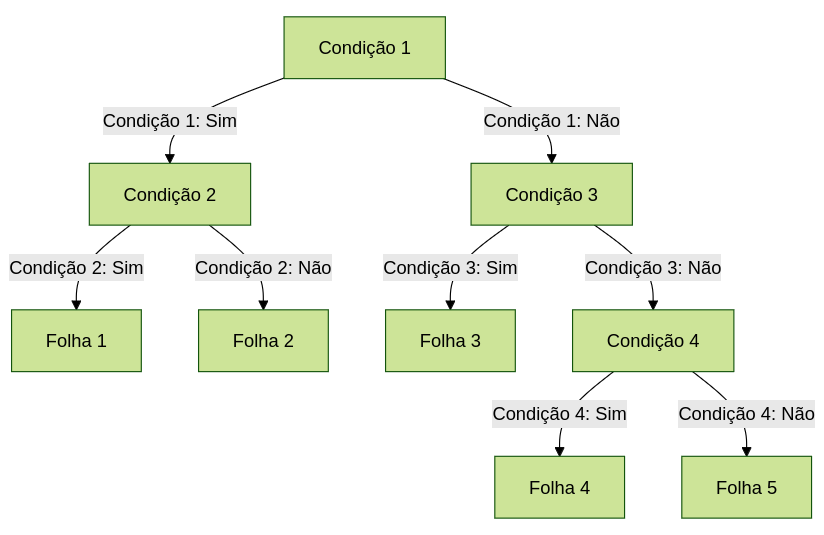
\includegraphics[keepaspectratio]{includes/mermaid-tree.png}}

}

\caption{\label{fig-arvore}Exemplo de estrutura de árvore de regressão.
A árvore tem cinco folhas e quatro nós internos.}

\end{figure}%

\vspace{12pt}

O espaço dos preditores é dividido em \(J\) regiões distintas e
disjuntas denotadas por \(R_1, R_2, \dots, R_J\). Essas regiões são
construídas em formato de caixa de forma a minimizar a soma dos
quadrados dos resíduos. Dessa forma, pode-se modelar a variável resposta
como uma constante \(c_j\) em cada região \(R_j\):

\[
f\left(x\right) = \sum^J_{j=1}c_j I\left(x \in R_j \right)\text{.}
\]

O estimador para a constante \(c_j\) é encontrado pelo método de mínimos
quadrados. Assim, deve-se minimizar
\(\sum_{x_i \in R_j} \left[y_i - f\left(x_i\right)\right]^2\). No
entanto, perceba que \(f\left(x_i\right)\) está sendo avaliado somente
em um ponto específico \(x_i\), o que reduzirá \(f\left(x_i\right)\)
para uma constante \(c_j\). É fácil de se chegar ao resultado se for
observada a definição da função indicadora \(I\left(x \in R_j\right)\):

\[
I_{R_j}(x_i) =
\begin{cases}
    1,& \text{se } x_i \in R_j \\
    0,& \text{se } x_i \notin R_j
\end{cases}\text{.}
\]

Como as regiões são disjuntas, \(x_i\) não pode estar simultaneamente em
duas regiões. Assim, para um ponto específico \(x_i\), apenas um dos
casos da função indicadora será diferente de 0. Portanto,
\(f\left(x_i\right) = c_j\). Agora, derivando
\(\sum_{x_i \in R_j}\left(yi - c_j\right)^2\) em relação a \(c_j\)

\begin{equation}\phantomsection\label{eq-partialdev}{
\frac{\partial}{\partial{c_j}}\sum_{x_i \in R_j} \left(y_i - c_j\right)^2 = -2\sum_{x_i \in R_j} \left(y_i - c_j\right)
}\end{equation} e, ao igualar a Equação~\ref{eq-partialdev} a 0, tem-se
a seguinte igualdade:

\[
\sum_{x_i \in R_j} \left(y_i - \hat{c}_j\right) = 0\text{.}
\]

Expandindo o somatório e dividindo pelo número total de pontos \(N_j\)
na região \(R_j\), concluí-se que o estimador de \(c_j\), denotado por
\(\hat{c}_j\), é simplesmente a média dos valores observados \(y_i\)
dentro da região \(R_j\):

\begin{equation}\phantomsection\label{eq-estimacjdev}{
\sum_{x_i \in R_j} y_i - \hat{c}_j N_j = 0 \Rightarrow \hat{c}_j = \frac{1}{N_{j}}\sum_{x_i \in R_j} y_i\text{.}
}\end{equation}

\vspace{12pt}

No entanto, JAMES et al. (2013) caracteriza como inviável considerar
todas as possíveis partições do espaço das variáveis em \(J\) caixas
devido ao alto custo computacional. Dessa forma, a abordagem a ser
adotada é uma divisão binária recursiva. O processo começa no topo da
árvore de regressão, o ponto em que contém todas as observações, e
continua sucessivamente dividindo o espaço dos preditores. As divisões
são indicadas como dois novos ramos na árvore, como pode ser visto na
Figura~\ref{fig-arvore}.

\vspace{12pt}

Para executar a divisão binária recursiva, deve-se primeiramente
selecionar a variável independente \(X_j\) e o ponto de corte \(s\) tal
que a divisão do espaço dos preditores conduza a maior redução possível
na soma dos quadrados dos resíduos. Dessa forma, definimos dois
semi-planos:

\[
R_{1}\left(j, s\right) = \{X | X_j \leq s\} \text{ e } R_{2}\left(j, s\right) = \{X | X_j > s\}\text{,}
\] e procuramos a divisão da variável \(j\) e o ponto de corte \(s\) que
minimizem a seguinte expressão:

\[
\min_{j, s}\left[\min_{c_1} \sum_{x_i \in R_1\left(j, s\right)} \left(y_i - c_{1}\right)^2 + \min_{c_2} \sum_{x_i \in R_2\left(j, s\right)} \left(y_i - c_{2}\right)^2\right]\text{,}
\] em que \(c_1\) e \(c_2\) é a média da variável dependente para as
observações nas regiões \(R_1\left(j, s\right)\) e
\(R_2\left(j, s\right)\), respectivamente. Após determinar a melhor
divisão, os dados são particionados nessas duas regiões, e o processo é
repetido recursivamente para todas as sub-regiões resultantes.

\vspace{12pt}

O tamanho da árvore pode ser considerado um hiperparâmetro para regular
a complexidade do modelo, pois uma árvore muito grande pode causar
sobreajuste aos dados de treinamento, capturando não apenas os padrões
relevantes, mas também o ruído. Como resultado, o modelo pode apresentar
bom desempenho nos dados de treinamento, mas falhar ao lidar com novos
dados devido à sua incapacidade de generalização. Por outro lado, uma
árvore muito pequena pode não captar padrões, relações e estruturas
importantes presentes nos dados. Dessa forma, a estratégia adotada para
selecionar o tamanho da árvore consiste em crescer uma grande árvore
\(T_0\), interrompendo o processo de divisão apenas ao atingir um
tamanho mínimo de nós. Posteriormente, a árvore \(T_0\) é podada
utilizando o critério de custo complexidade, que será definido a seguir.

\vspace{12pt}

Para o processo de poda da árvore, definimos uma árvore qualquer \(T\)
que pode ser obtida através do processo da poda de \(T_0\), de modo que
\(T \subset T_0\). Assim, sendo \(N_j\) a quantidade de pontos na região
\(R_j\), seja

\[
Q_j\left(T\right) = \frac{1}{N_j} \sum_{x_i \in R_j}\left(y_i - \hat{c}_j\right)^2
\] uma medida de impureza do nó pelo erro quadrático médio. Assim,
define-se o critério de custo complexidade:

\[
C_{\alpha}\left(T\right) = \sum_{m = 1}^{|T|}N_jQ_j\left(T\right) + \alpha |T|\text{,}
\] em que \(|T|\) denota a quantidade total de folhas, e
\(\alpha \geq 0\) é um hiperparâmetro que equilibra o tamanho da árvore
e a adequação aos dados. A ideia é encontrar, para cada \(\alpha\), a
árvore \(T_{\alpha} \subset T_0\) que minimiza
\(C_{\alpha}\left(T\right)\). Valores grandes de \(\alpha\) resultam em
árvores menores, enquanto valores menores resultam em árvores maiores, e
\(\alpha = 0\) resulta na própria árvore \(T_0\). A busca por
\(T_{\alpha}\) envolve colapsar sucessivamente o nó interno que provoca
o menor aumento em \(\sum_j N_j Q_j\left(T\right)\), continuando o
processo até produzir uma árvore com um único nó. Esse processo gera uma
sequência de subárvores, na qual existe uma única subárvore menor que,
para cada \(\alpha\), minimiza \(C_{\alpha}\left(T\right)\).

\vspace{12pt}

A estimação de \(\alpha\) pode ser realizada por validação cruzada com
cinco ou dez folds, sendo \(\hat \alpha\) escolhido para minimizar a
soma dos quadrados dos resíduos durante o processo de validação cruzada.
Assim, a árvore final será \(T_{\hat \alpha}\). O
 Algoritmo~\ref{algo-buildtree}  exemplifica o processo de crescimento
de uma árvore de regressão:

\begin{algo}

\centering{

\begin{algorithm}[H]
\caption{Algoritmo para crescer uma árvore de regressão.}
\begin{algorithmic}
\State \textbf{1.} Use a divisão binária recursiva para crescer uma árvore grande $T_0$ nos dados de treinamento, parando apenas quando cada folha tiver menos do que um número mínimo de observações.

\vspace{3.7pt}

\State \textbf{2.} Aplique o critério custo de complexidade à árvore grande \( T_0 \) para obter uma sequência de melhores subárvores \( T_\alpha \), em função de \( \alpha \).

\vspace{3.7pt}

\State \textbf{3.} Use validação cruzada $K\text{-fold}$ para escolher \( \alpha \). Isto é, divida as observações de treinamento em $K$ folds. Para cada \( k = 1, \ldots, K \):
    \State \hspace{1em} (a) Repita os Passos 1 e 2 em todos os folds, exceto no $k\text{-ésimo}$ fold dos dados de
    \State \hspace{1em} treinamento.
    \State \hspace{1em} (b) Avalie o erro quadrático médio da previsão no $k\text{-ésimo}$ fold deixado
    \State \hspace{1em} de fora, em função de \( \alpha \).

    \vspace{3pt}

    \State \hspace{1em} Faça a média dos resultados para cada valor de \( \alpha \) e escolha \( \alpha \) que minimize o erro
    \State \hspace{1em} médio.

\vspace{3.7pt}

\State \textbf{4.} Retorne a subárvore \( T_{\hat{\alpha}} \) do Passo 2 que corresponde ao valor estimado de \( \alpha \).
\end{algorithmic}
\end{algorithm}

}

\caption{\label{algo-buildtree}Fonte: JAMES et al. (2013, p. 337).}

\end{algo}%

\vspace{12pt}

No caso de uma árvore de decisão para classificação, a principal
diferença está no critério de divisão dos nós e na poda da árvore. Para
a classificação, a previsão em um nó \(j\), correspondente a uma região
\(R_j\) com \(N_j\) observações, será simplesmente a classe majoritária.
Assim, tem-se:

\[
\hat{p}_{jk} = \frac{1}{N_j}\sum_{x_i \in R_j} I\left(y_i = k\right)\text{,}
\] como sendo a proporção de observações da classe \(k\) no nó \(j\).
Dessa forma, as observações no nó \(j\) são classificadas na classe
\(k\left(j\right) = \arg \max_{k} \hat{p}_{jk}\), que é a moda no nó
\(j\).

\vspace{12pt}

Para a divisão dos nós no caso da regressão, foi utilizado o erro
quadrático médio como medida de impureza. Para a classificação, algumas
medidas comuns para \(Q_j\left(T\right)\) são o erro de classificação, o
índice de Gini ou a entropia cruzada.

\section{Métodos Ensemble}\label{muxe9todos-ensemble}

~~~As árvores de decisão são conhecidas por sua alta interpretabilidade,
mas geralmente apresentam um desempenho preditivo inferior em comparação
com outros modelos e algoritmos. No entanto, é possível superar essa
limitação construindo um modelo preditivo que combina a força de uma
coleção de estimadores base, um processo conhecido como aprendizado em
conjunto (Ensemble Learning). De acordo com HASTIE et al. (2009), o
aprendizado em conjunto pode ser dividido em duas etapas principais: a
primeira etapa consiste em desenvolver uma população de algoritmos de
aprendizado base a partir dos dados de treinamento, e a segunda etapa
envolve a combinação desses algoritmos para formar um estimador
agregado. Portanto, nesta seção, serão definidos os métodos de
aprendizado em conjunto utilizados neste trabalho.

\subsection{Random Forest}\label{random-forest}

\begin{algo}

\centering{

\begin{algorithm}[H]
\caption{Algoritmo de uma Random Forest para regressão ou classificação.}
\begin{algorithmic}
\State \hspace{1em} \textbf{1.} Para b = 1 até B:

\vspace{0.8em}

    \State \hspace{2em} (a) Construa amostras bootstrap $\mathbf{\mathcal{L}}^*$ de tamanho \( N \) dos dados de
    \State \hspace{3.6em} \vspace{0.1em} treinamento.

    \State \hspace{2em} (b) Faça crescer uma árvore de floresta aleatória \( T_b \) para os dados bootstrap,
    \State \hspace{3.6em} repetindo recursivamente os seguintes passos para cada folha da árvore,
    \State \hspace{3.6em} \vspace{0.5em} até que o tamanho mínimo do nó \( n_{min} \) seja atingido:
    \State \hspace{4em} \vspace{0.1em} i. Selecione \( m \) variáveis aleatoriamente entre as \( p \) variáveis.
    \State \hspace{4em} \vspace{0.1em} ii. Escolha a melhor variável entre as \( m \).
    \State \hspace{4em} \vspace{0.1em} iii. Divida o nó em dois subnós.

\vspace{0.8em}

\State \hspace{1em} \textbf{2.} Por fim, o conjunto de árvores \( \{T_b\}^{B}_1\) é construído.

\vspace{1em}

\State \hspace{0.7em} No caso da regressão, para fazer uma predição em um novo ponto \( x \), temos a seguinte função:


$$
\hat{f}^{B}_{rf}\left(x\right) = \frac{1}{B}\sum^{B}_{b = 1} T_{b}\left(x\right)
$$

\vspace{1em}

\State \hspace{0.7em} Para a classificação é utilizado o voto majoritário. Assim, seja $\hat{C}_{b}\left(x\right)$ a previsão da classe da árvore de floresta aleatória $b$. Assim:

$$
\hat{C}^{B}_{rf}\left(x\right) = \arg \max_c \sum^{B}_{b = 1}I\left(\hat{C}_b\left(x\right) = c\right)\text{,}
$$

\State em que $c$ representa as classes possíveis.

\end{algorithmic}
\end{algorithm}

}

\caption{\label{algo-rf}Fonte: HASTIE et al. (2009, p. 588).}

\end{algo}%

~~~O algoritmo Random Forest é uma técnica derivada do método de
Bagging, mas com modificações específicas na construção das árvores. O
objetivo é melhorar a redução da variância ao diminuir a correlação
entre as árvores, sem aumentar significativamente a variabilidade. Isso
é alcançado durante o processo de crescimento das árvores por meio da
seleção aleatória de variáveis independentes.

\vspace{12pt}

No algoritmo Random Forest, ao construir uma árvore a partir de amostras
bootstrap, selecionam-se aleatoriamente \(m \leq p\) das \(p\) variáveis
independentes como candidatas para a divisão, antes de cada ramificação
(com \(m = p\) no caso do Bagging). Dessa forma, diferente do Bagging,
aqui não se considera todas as \(p\) variáveis independentes para
realizar a divisão e minimizar a impureza, mas apenas \(m\) dessas \(p\)
variáveis. A escolha aleatória de apenas \(m\) covariáveis como
candidatas para a divisão ajuda a solucionar um dos principais problemas
do algoritmo de Bagging, que tende a gerar árvores de decisão
semelhantes, resultando em previsões altamente correlacionadas. O Random
Forest busca diminuir esse problema ao criar oportunidades para que
diferentes preditores sejam considerados. Em média, uma fração
\((p -m)/ p\) das divisões nem sequer incluirá o preditor mais forte
como candidato, permitindo que outros preditores tenham a chance de
serem selecionados (JAMES et al., 2013). Esse mecanismo reduz a
correlação entre as árvores, o que, por sua vez, diminui a variabilidade
das predições produzidas pelas árvores.

\vspace{12pt}

A quantidade de variáveis independentes \(m\) selecionadas
aleatoriamente é um hiperparâmetro que pode ser estimado por meio de
validação cruzada. Valores comuns para \(m\) são
\(m=\sqrt{p}\)\hspace{0pt} com tamanho mínimo do nó igual a um para
classificação, e \(m=p/3\)\hspace{0pt} com tamanho mínimo do nó igual a
cinco para regressão (HASTIE et al., 2009). Quando o número de variáveis
é grande, mas poucas são realmente relevantes, o algoritmo Random Forest
pode ter um desempenho inferior com valores pequenos de \(m\), pois isso
reduz as chances de selecionar as variáveis mais importantes. No
entanto, usar um valor pequeno de \(m\) pode ser vantajoso quando há
muitos preditores correlacionados. Além disso, assim como no Bagging, a
Random Forest não sofre de sobreajuste com o aumento da quantidade de
árvores \(B\). Portanto, é suficiente usar um \(B\) grande o bastante
para que a taxa de erro se estabilize (JAMES et al., 2013).

\textbf{(FALAR SOBRE O EXTRA TREES)}

\section{Modelos de séries
temporais}\label{modelos-de-suxe9ries-temporais}

\subsection{Suavização exponencial sazonal de
Holt-Winters}\label{suavizauxe7uxe3o-exponencial-sazonal-de-holt-winters}

~~~O método de suavização exponencial de Holt-Winters (HW) é uma
extensão da suavização exponencial simples para séries temporais que
apresentam tendência e sazonalidade. Esse método baseia-se em três
equações, cada uma com uma constante de suavização distinta, associadas
às três componentes fundamentais da série: nível, tendência e
sazonalidade (MORETTIN; TOLOI, 2022).

\vspace{12pt}

Considerando uma série com sazonalidade de período \(s\), a forma mais
comum do método assume um componente sazonal multiplicativo e uma
tendência aditiva. Nesse caso, a série é modelada por:

\[
Z_t = \mu_{t} F_{t} + T_{t} + a_{t}, t = 1, \cdots, N.
\]

As três equações de suavização associadas ao fator sazonal, ao nível e à
tendência são, respectivamente:

\[
\begin{aligned}
\hat{F}_{t} &= D \left(\frac{Z_{t}}{\bar{Z}_{t}}\right) + \left(1 - D\right) \hat{F}_{t-s}, \ 0 < D< 1, \ t = s + 1, \cdots, N \text{, } \\
\bar{Z}_{t} &= A \left(\frac{Z_{t}}{\hat{F}_{t-s}}\right) + \left(1 - A\right)\left(\hat{Z}_{t-1} + \hat{T}_{t-1}\right), \ 0<A<1, \ t = s+1,\cdots, N \text{, } \\
\hat{T}_{t} &= C\left(\bar{Z}_{t} - \bar{Z}_{t -1}\right) + \left(1 - C\right)\hat{T}_{t - 1}, \ 0< C <1, \ t=s+1, \cdots, N
\end{aligned}
\]

As constantes \(A\), \(C\) e \(D\) representam os parâmetros de
suavização do nível, da tendência e da sazonalidade, respectivamente. A
previsão futura dos valores, nesse caso, é dada por:

\[
\hat{Z}_{t+1}\left(h - 1\right) = \left(\bar{Z}_{t+1} + \left(h - 1\right)\hat{T}_{t+1}\right)\hat{F}_{t+1+h - s} \text{, } h = 1, 2, \cdots, s + 1
\]

\vspace{12pt}

No caso em que o fator sazonal é aditivo, o modelo assume a forma:

\[
Z_{t} = \mu_{t} + T_{t} + F_{t} + a_{t}.
\]

As equações de suavização para o componente sazonal, o nível e a
tendência, respectivamente, tornam-se:

\[
\begin{aligned}
\hat{F}_{t} &= D \left(Z_{t} - \bar{Z}_{t}\right) + \left(1 - D\right) \hat{F}_{t-s}, \ 0 < D< 1 \text{, } \\
\bar{Z}_{t} &= A \left(Z_{t} - \hat{F}_{t-s}\right) + \left(1 - A\right)\left(\bar{Z}_{t-1} + \hat{T}_{t-1}\right), \ 0<A<1 \text{, } \\
\hat{T}_{t} &= C\left(\bar{Z}_{t} - \bar{Z}_{t -1}\right) + \left(1 - C\right)\hat{T}_{t - 1}, \ 0< C <1 \text{, }
\end{aligned}
\]

Por fim, a previsão dos valores futuros para o caso aditivo é dada por:

\[
\hat{Z}_{t+1}\left(h - 1\right) = \bar{Z}_{t + 1} + \left(h - 1\right)\hat{T}_{t+1}+\hat{F}_{t + 1 + h - s}, \ h=1,\cdots, s+1 \text{.}
\]

\subsection{LSTM}\label{lstm}

\subsection{ARIMA}\label{arima}

~~~Os modelos de séries temporais da classe ARIMA estão entre os mais
utilizados na modelagem de dados temporais. Seu principal objetivo é
descrever as autocorrelações presentes nos dados.

\vspace{12pt}

Os modelos ARIMA são compostos por dois componentes fundamentais: o
modelo autorregressivo (AR) e o modelo de médias móveis (MA). O modelo
autorregressivo utiliza uma combinação linear de valores passados da
variável. Assim, um modelo AR de ordem \(p\) pode ser escrito como:

\[
y_{t} = c + \phi_{1}y_{t-1} + \phi_{2}y_{t-2} + \cdots + \phi_{p}y_{t-p} + \epsilon_{t}\text{, }
\] em que \(\epsilon_{t}\) representa o ruído branco. O modelo
autorregressivo de ordem \(p\) é denotado por
\(\text{AR}\left(p\right)\).

\vspace{12pt}

Por sua vez, o modelo de médias móveis de ordem \(q\), denotado por
\(\text{MA}\left(q\right)\), utiliza erros passados para prever os
valores futuros da série. Ele é expresso por:

\[
y_{t} = c + \epsilon_{t} + \theta_{1}\epsilon_{t - 1} + \theta_{2}\epsilon_{t-2} + \cdots + \theta_{q}\epsilon_{t-q}\text{.}
\]

A partir da combinação dos modelos AR e MA, tem-se o modelo ARIMA, cuja
estrutura incorpora também a diferenciação da série temporal para
torná-la estacionária. O modelo ARIMA é dado por:

\[
y^{'}_{t} = c + \phi_{1}y^{'}_{t-1} + \cdots + \phi_{p}y^{'}_{t-p} + \theta_{1}\epsilon_{t-1}+ \cdots + \theta_{q}\epsilon_{t-q} + \epsilon_{t}\text{, }
\] em que \(y^{'}_t\) representa a série temporal após ter sido
diferenciada (possivelmente mais de uma vez). O modelo é denotado por
\(\text{ARIMA}\left(p, d, q\right)\), em que \(p\) é a ordem da
componente autorregressiva, \(d\) é o número de diferenciações aplicadas
e \(q\) é a ordem da componente de médias móveis.

\vspace{12pt}

O modelo ARIMA apresentado anteriormente aplica-se ao caso em que não há
sazonalidade. No entanto, os modelos ARIMA também podem ser estendidos
para séries temporais com padrão sazonal. Nessa situação, são incluídas
componentes sazonais adicionais, resultando no modelo sazonal ARIMA,
denotado por:

\[
\text{ARIMA}\left(p, d, q\right)\left(P, D, Q\right)_m
\] em que \(m\) representa o período da sazonalidade (por exemplo, o
número de observações por ano), e \(P\), \(D\) e \(Q\) correspondem,
respectivamente, às ordens das componentes autorregressiva, de
diferenciação e de médias móveis para a parte sazonal do modelo.

\section{Elastic-Net}\label{elastic-net}

~~~O modelo de Elastic-Net combina dois tipos de regressão com
penalização, o Lasso e o Ridge, que servem para reduzir os coeficientes
de regressão linear.

\vspace{12pt}

A regressão Ridge é um tipo de regressão que busca controlar os
coeficientes impondo uma penalidade aos seus valores. Quando existem
múltiplas variáveis correlacionadas em um modelo de regressão linear, os
coeficientes podem exibir alta variância. Um coeficiente altamente
positivo em uma variável pode ser cancelado por um altamente negativo em
outra variável correlacionada. O objetivo da regressão Ridge é mitigar
esse problema.

\vspace{12pt}

A regressão ridge é muito semelhante aos mínimos quadrados, exceto que
os coeficientes são estimados minimizando uma quantidade ligeiramente
diferente. Em particular, as estimativas do coeficiente de regressão de
ridge \(\hat{\beta}^{\text{ridge}}\) são os valores que minimizam

\[
\hat{\beta}^{\text{ridge}} = \arg \min_{\beta} \Biggl\{\sum_{i = 1}^{n}\left(y_{i} - \beta_{0} - \sum_{j=1}^{p}x_{ij}\beta_{j}\right)^2 + \lambda \sum_{j=1}^{p}\beta_{j}^2 \Biggl\}\text{, }
\] em que \(\lambda \geq 0\) é um parâmetro de ajuste, a ser determinado
separadamente.

\vspace{12pt}

Assim como com os mínimos quadrados, a regressão ridge busca estimativas
de coeficientes que se ajustem bem aos dados, tornando o soma dos
quadrados dos erros pequeno. No entanto, o segundo termo,
\(\lambda \sum_{j=1}^{p}\beta_{j}^2\), chamado de penalidade de
encolhimento (shrinkage penalty), é pequeno quando
\(\beta_{1}, \cdots, \beta_{p}\) estão próximos de zero e, portanto, tem
o efeito de encolher as estimativas de \(\beta_j\) em direção a zero. O
parâmetro de ajuste \(\lambda\) serve para controlar o impacto relativo
desses dois termos nas estimativas do coeficiente de regressão.

\vspace{12pt}

Quando \(\lambda = 0\), o termo de penalidade não tem efeito e a
regressão ridge produzirá as estimativas dos mínimos quadrados. No
entanto, conforme \(\lambda \rightarrow \infty\), o impacto da
penalidade de encolhimento aumenta e as estimativas do coeficiente de
regressão ridge se aproximarão de zero.

\vspace{12pt}

Na regressão lasso, a soma dos mínimos quadrados penalizada é dada por:

\[
\hat{\beta}^{\text{lasso}} = \arg \min_{\beta} \Biggl\{\frac{1}{2}\sum_{i = 1}^{n}\left(y_{i} - \beta_{0} - \sum_{j=1}^{p}x_{ij}\beta_{j}\right)^2 + \lambda \sum_{j=1}^{p}|\beta_{j}| \Biggl\}\text{, }
\] em que um valor de \(\lambda\) suficientemente grande fará com que
alguns coeficientes sejam exatamente 0.

\vspace{12pt}

A regressão Lasso tem algumas limitações. Em problemas com \(p\) grande
e \(n\) pequeno, a regressão lasso selecionará no máximo \(n\)
variáveis. Além disso, em um grupo de variáveis muito correlacionadas, a
lasso tende a selecionar apenas uma variável do grupo.

\vspace{12pt}

Para solucionar essas limitações a regressão elastic net adiciona a
penalização quadrática da ridge à penalização da lasso. Dessa forma, o
problema então torna-se:

\[
\hat{\beta} = \arg \min_{\beta} \Biggl\{\frac{1}{2}\sum_{i = 1}^{n}\left(y_{i} - \beta_{0} - \sum_{j=1}^{p}x_{ij}\beta_{j}\right)^2 + \lambda_{2} \sum_{j=1}^{p}\beta_{j}^2 + \lambda_{1} \sum_{j=1}^{p}|\beta_{j}| \Biggl\}\text{, }
\]

\vspace{12pt}

Com \(\lambda_{1} = 0\), temos ridge, com \(\lambda_{2} = 0\), temos
lasso e com \(\lambda_{1} = \lambda_{2} = 0\), temos regressão linear
sem regularização.

\chapter{Metodologia}\label{metodologia}

\chapter{Produto final}\label{produto-final}

\chapter{Conclusão}\label{conclusuxe3o}

\chapter*{\texorpdfstring{\centering Referências}{Referências}}\label{referuxeancias}

\markboth{Referências}{Referências}

\phantomsection\label{refs}
\begin{CSLReferences}{0}{1}
\bibitem[\citeproctext]{ref-optuna_2019}
AKIBA, T. et al. Optuna: A Next-generation Hyperparameter Optimization
Framework. {[}S.l.{]}: {[}s.n.{]}, 2019.

\bibitem[\citeproctext]{ref-quarto}
ALLAIRE, J.; DERVIEUX, C.
\textbf{\href{https://CRAN.R-project.org/package=quarto}{quarto: R
Interface to 'Quarto' Markdown Publishing System}}. {[}S.l.{]}:
{[}s.n.{]}, 2024.

\bibitem[\citeproctext]{ref-sqlalchemy}
BAYER, M. \href{http://aosabook.org/en/sqlalchemy.html}{SQLAlchemy}.
\emph{Em}: BROWN, A.; WILSON, G. (Org.). \textbf{The Architecture of
Open Source Applications Volume II: Structure, Scale, and a Few More
Fearless Hacks}. {[}S.l.{]}: aosabook.org, 2012.

\bibitem[\citeproctext]{ref-chen2016xgboost}
CHEN, T.; GUESTRIN, C. Xgboost: A scalable tree boosting system.
{[}S.l.{]}: {[}s.n.{]}, 2016. p. 785--794.

\bibitem[\citeproctext]{ref-harris2020array}
HARRIS, C. R. et al. Array programming with {NumPy}. \textbf{Nature},
set. 2020. v. 585, n. 7825, p. 357--362. Disponível em:
\textless{}\url{https://doi.org/10.1038/s41586-020-2649-2}\textgreater.

\bibitem[\citeproctext]{ref-hastie2009elements}
HASTIE, T. et al. \textbf{The elements of statistical learning: data
mining, inference, and prediction}. {[}S.l.{]}: Springer, 2009. V. 2.

\bibitem[\citeproctext]{ref-shammamah_hossain-proc-scipy-2019}
HOSSAIN, Shammamah.
\href{https://doi.org/10.25080/Majora-7ddc1dd1-012}{{V}isualization of
{B}ioinformatics {D}ata with {D}ash {B}io}. (Chris Calloway et al.,
Org.). {[}S.l.{]}: {[}s.n.{]}, 2019. p. 126--133.

\bibitem[\citeproctext]{ref-Hunter:2007}
HUNTER, J. D. \href{https://doi.org/10.1109/MCSE.2007.55}{Matplotlib: A
2D graphics environment}. \textbf{Computing in Science \& Engineering},
2007. v. 9, n. 3, p. 90--95.

\bibitem[\citeproctext]{ref-plotly}
INC., P. T. Collaborative data science. 2015. Disponível em:
\textless{}\url{https://plot.ly}\textgreater.

\bibitem[\citeproctext]{ref-james2013introduction}
JAMES, G. et al. \textbf{An introduction to statistical learning}.
{[}S.l.{]}: Springer, 2013. V. 112.

\bibitem[\citeproctext]{ref-ke2017lightgbm}
KE, G. et al. Lightgbm: A highly efficient gradient boosting decision
tree. \textbf{Advances in neural information processing systems}, 2017.
v. 30.

\bibitem[\citeproctext]{ref-NIPS2017_7062}
LUNDBERG, S. M.; LEE, S.-I.
\href{http://papers.nips.cc/paper/7062-a-unified-approach-to-interpreting-model-predictions.pdf}{A
Unified Approach to Interpreting Model Predictions}. \emph{Em}: GUYON,
I. et al. (Org.). \textbf{Advances in Neural Information Processing
Systems 30}. {[}S.l.{]}: Curran Associates, Inc., 2017, p. 4765--4774.

\bibitem[\citeproctext]{ref-morettin2022analise}
MORETTIN, P. A.; TOLOI, C. M. De C. An{á}lise de s{é}ries temporais.
2022.

\bibitem[\citeproctext]{ref-scikit-learn}
PEDREGOSA, F. et al. Scikit-learn: Machine Learning in {P}ython.
\textbf{Journal of Machine Learning Research}, 2011. v. 12, p.
2825--2830.

\bibitem[\citeproctext]{ref-folium}
PYTHON-VISUALIZATION. \textbf{Folium}. Disponível em:
\textless{}\url{https://python-visualization.github.io/folium/}\textgreater.

\bibitem[\citeproctext]{ref-reback2020pandas}
TEAM, T. Pandas Development. \textbf{pandas-dev/pandas: Pandas}. Zenodo.
Disponível em:
\textless{}\url{https://doi.org/10.5281/zenodo.3509134}\textgreater.

\bibitem[\citeproctext]{ref-2020SciPy-NMeth}
VIRTANEN, P. et al.
\href{https://doi.org/10.1038/s41592-019-0686-2}{{{SciPy} 1.0:
Fundamental Algorithms for Scientific Computing in Python}}.
\textbf{Nature Methods}, 2020. v. 17, p. 261--272.

\bibitem[\citeproctext]{ref-Waskom2021}
WASKOM, M. L. seaborn: statistical data visualization. \textbf{Journal
of Open Source Software}, 2021. v. 6, n. 60, p. 3021. Disponível em:
\textless{}\url{https://doi.org/10.21105/joss.03021}\textgreater.

\end{CSLReferences}




\end{document}
